\documentclass[
    a4paper,
    doc,
    british
]{apa6}

\usepackage[british]{babel}
\usepackage[utf8]{inputenc}
\usepackage{epstopdf}
\usepackage{csquotes}
\usepackage[hidelinks]{hyperref}
\usepackage{graphicx}

\usepackage[
    style=apa,
    backend=biber,
    sortcites=true,
    sorting=nyt,
%    isbn=false,
%    url=false,
%    doi=false,
%    eprint=false,
    hyperref=false,
    backref=false,
%    firstinits=false,
]{biblatex}

\DeclareLanguageMapping{british}{british-apa}

%%%%%%%%%%%%%%%%%%%%%%%%%%%%%%%%%%%%%%%%%%%%%%%%%%%

\title{CSCD01W20 Team 4 Development Team Biographies}
\shorttitle{Team 4 Developer Biographies}
\author{Team 4}
\affiliation{CSCD01W20\\
University of Toronto\\
Department of Computer and Mathematical Sciences}

\begin{document}

\maketitle

\newpage

\section{Team 4}

We are cool. Get to know us!

\newpage
\section[Joe]{Joe Armitage}

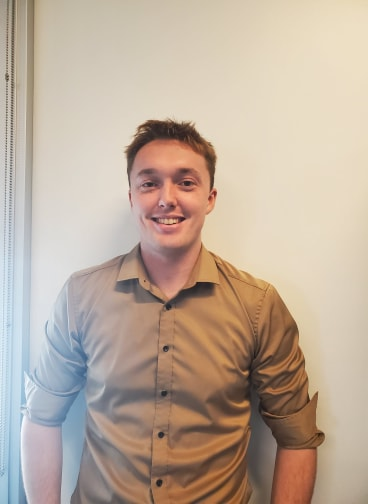
\includegraphics[width=0.5\textwidth]{pic/joe}

\subsection[CV]{Curriculum Vitae}

I like turtles.

\subsection[Role]{Primary Role as Developer of Project}

I want to code... good.

\newpage
\section[Joe]{Joe Armitage}

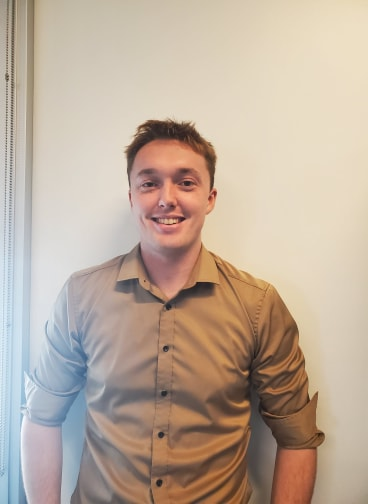
\includegraphics[width=0.5\textwidth]{pic/joe}

\subsection[CV]{Curriculum Vitae}

I like turtles.

\subsection[Role]{Primary Role as Developer of Project}

I want to code... good.

\newpage
\section[Joe]{Joe Armitage}

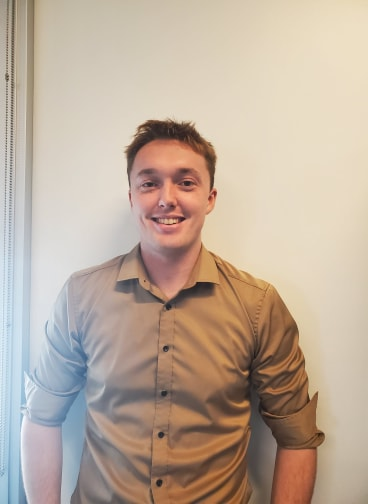
\includegraphics[width=0.5\textwidth]{pic/joe}

\subsection[CV]{Curriculum Vitae}

I like turtles.

\subsection[Role]{Primary Role as Developer of Project}

I want to code... good.

\newpage
\section[Joe]{Joe Armitage}

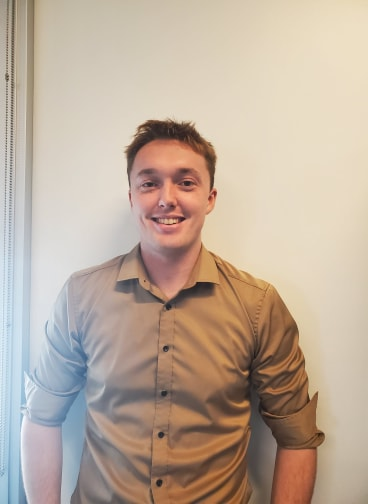
\includegraphics[width=0.5\textwidth]{pic/joe}

\subsection[CV]{Curriculum Vitae}

I like turtles.

\subsection[Role]{Primary Role as Developer of Project}

I want to code... good.

\newpage
\section[Angela]{Angela Zavaleta}

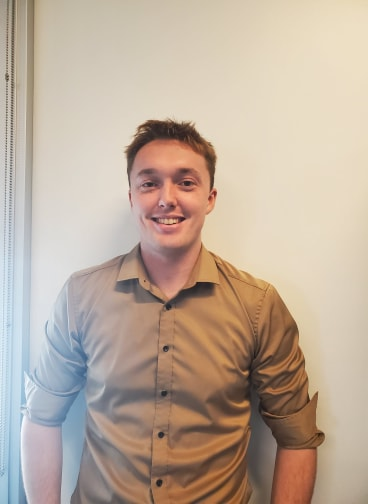
\includegraphics[width=0.5\textwidth]{pic/joe}

\subsection[CV]{Curriculum Vitae}

I like turtles.

\subsection[Role]{Primary Role as Developer of Project}

I want to code... good.

\newpage

\appendix
\input{appendix}

\end{document}
